% Supplementary material. Same fallback note as main.tex: swap the two marked
% lines for \documentclass[sn-mathphys-num]{sn-jnl} when sn-jnl.cls is available.
\documentclass[pdflatex,sn-basic]{sn-jnl}
\pdfmapfile{=local.map}          %% build-machine workaround; delete elsewhere
\usepackage{graphicx}%
\usepackage{multirow}%
\usepackage{amsmath,amssymb,amsfonts}%
\usepackage{amsthm}%
\usepackage{mathrsfs}%
\usepackage[title]{appendix}%
\usepackage{xcolor}%
\usepackage{textcomp}%
\usepackage{manyfoot}%
\usepackage{booktabs}%

\renewcommand{\thefigure}{S\arabic{figure}}
\renewcommand{\thetable}{S\arabic{table}}

\begin{document}

\title{Supplementary Material\\
       \large Does Synthetic Data Preserve Cluster Structure?
       A Factorial Evaluation of Partitioning and Hierarchical
       Clustering on {CART}-Generated Data}
\author[1]{Oriol Farr\'es Vilar}
\author[1,2]{Jordi Cort\'es}
\author[2]{Daniel Fern\'andez}
\affil[1]{Universitat Polit\`ecnica de Catalunya, Barcelona, Spain}
\affil[2]{Universitat Polit\`ecnica de Catalunya, Barcelona, Spain}
\abstract{Supporting figures and tables for the main article.}
\maketitle

\section{Recovery of the number of groups by cluster count and separation}

Figure~\ref{figS:heatmap} presents the recovery rate of the true number of
groups as a function of the true cluster count $k$ and the separation
$\sigma$, for both algorithms. It carries the same information as Figure~3 of
the main article in a different layout, making the $k \times \sigma$
interaction directly legible: recovery collapses in the lower-left quadrant
(many groups, little separation) and is essentially perfect in the upper-right.

\begin{figure}[h]
\centering
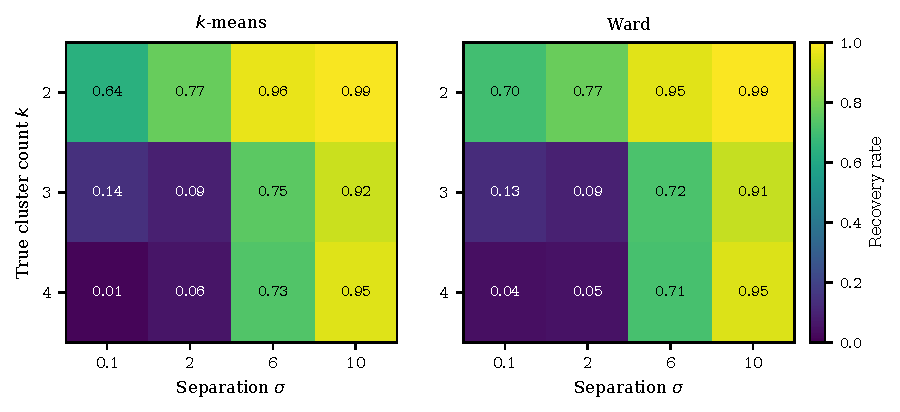
\includegraphics[width=\textwidth]{figures/figS_heatmap.pdf}
\caption{Recovery rate of the true number of groups by true cluster count and
  separation, for $k$-means (left) and Ward (right). Cell values are
  proportions over the full design.}
\label{figS:heatmap}
\end{figure}

\section{Agreement in the estimated number of groups between original and
         synthetic data}

Table~\ref{tabS:khat} cross-tabulates the number of groups estimated from the
original data against the number estimated from the corresponding synthetic
data, stratified by separation. Unlike the recovery rate in the main article,
which scores $\hat{k}$ against the construction-time ground truth, this table
compares the two estimates with each other and so isolates the effect of
synthesis from the difficulty of the clustering problem itself.

The pattern confirms the expectation that at high separation the mass
concentrates on the diagonal: exact agreement rises from $68.4\%$ at
$\sigma = 0.1$ to $98.2\%$ at $\sigma = 10$ for $k$-means (Ward: $64.6\%$ to
$97.5\%$). In the overlapping regime the off-diagonal mass is not symmetric.
At $\sigma = 0.1$ the synthetic data yield a \emph{lower} estimate than the
original in $15.2\%$ of comparisons and a higher one in $16.4\%$; the largest
single off-diagonal cell is the original data supporting $\hat{k} \ge 5$ while
the synthetic data support $\hat{k} = 2$ ($8.4\%$). That is, when the original
data contain weak, diffuse structure that the silhouette criterion resolves
into many small groups, CART synthesis tends to smooth it away into a single
coarse split. The tendency disappears once the groups are genuinely separated.

\begin{table}[h]
\centering
\caption{Agreement in the estimated number of groups between original and
  synthetic data, by separation. Rows are $\hat{k}$ from the original data,
  columns $\hat{k}$ from the synthetic data; cells are percentages of all
  comparisons at that separation (each block sums to $100\%$). Estimates of
  five or more groups are pooled for display, but the agreement column is
  computed on unpooled values. Both data sources are searched over a fixed
  range $\hat{k} \in \{2,\dots,8\}$, so the comparison is symmetric; under the
  narrower per-scenario range used for the recovery rates in the main text,
  agreement is higher in the overlapping regime ($75.1\%$ and $67.6\%$ at
  $\sigma = 0.1$, $79.7\%$ and $75.9\%$ at $\sigma = 2$, for $k$-means and Ward
  respectively) and essentially unchanged at $\sigma \ge 6$, where the two
  conventions differ by at most $0.1$ percentage points.
  $n = 180{,}000$ comparisons per separation level.}
\label{tabS:khat}
\small
\begin{tabular}{llrrrrr}
\toprule
 & & \multicolumn{4}{c}{$\hat{k}$ recovered from synthetic data (\%)} & Exact \\
\cmidrule(lr){3-6}
$\sigma$ & $\hat{k}$ (original) & 2 & 3 & 4 & $\geq 5$ & agreement \\
\midrule
\multicolumn{7}{l}{\textit{$k$-means}} \\
\multirow{4}{*}{0.1} & 2 & 50.8 & 2.0 & 0.5 & 3.8 & \multirow{4}{*}{$68.2\%$} \\
 & 3 & 2.1 & 10.1 & 0.5 & 4.0 &  \\
 & 4 & 0.0 & 0.0 & 0.0 & 0.0 &  \\
 & $\geq 5$ & 8.6 & 1.0 & 0.7 & 15.8 &  \\
\addlinespace
\multirow{4}{*}{2} & 2 & 62.8 & 3.3 & 1.7 & 4.4 & \multirow{4}{*}{$76.6\%$} \\
 & 3 & 1.2 & 8.8 & 0.7 & 2.1 &  \\
 & 4 & 0.3 & 0.3 & 0.9 & 1.3 &  \\
 & $\geq 5$ & 2.4 & 0.9 & 1.0 & 8.0 &  \\
\addlinespace
\multirow{4}{*}{6} & 2 & 38.0 & 1.0 & 0.3 & 0.1 & \multirow{4}{*}{$92.5\%$} \\
 & 3 & 0.7 & 29.1 & 1.1 & 0.1 &  \\
 & 4 & 0.5 & 2.4 & 24.7 & 0.8 &  \\
 & $\geq 5$ & 0.0 & 0.1 & 0.1 & 0.8 &  \\
\addlinespace
\multirow{4}{*}{10} & 2 & 34.8 & 0.1 & 0.1 & 0.4 & \multirow{4}{*}{$98.3\%$} \\
 & 3 & 0.3 & 31.7 & 0.2 & 0.0 &  \\
 & 4 & 0.0 & 0.2 & 31.8 & 0.2 &  \\
 & $\geq 5$ & 0.0 & 0.0 & 0.0 & 0.0 &  \\
\addlinespace
\midrule
\multicolumn{7}{l}{\textit{Ward}} \\
\multirow{4}{*}{0.1} & 2 & 58.4 & 5.0 & 2.0 & 6.8 & \multirow{4}{*}{$64.9\%$} \\
 & 3 & 3.5 & 4.9 & 0.9 & 3.4 &  \\
 & 4 & 1.0 & 1.1 & 0.3 & 0.9 &  \\
 & $\geq 5$ & 6.2 & 1.4 & 0.6 & 3.4 &  \\
\addlinespace
\multirow{4}{*}{2} & 2 & 65.6 & 4.6 & 2.2 & 5.4 & \multirow{4}{*}{$73.8\%$} \\
 & 3 & 1.1 & 6.5 & 1.0 & 2.0 &  \\
 & 4 & 1.1 & 0.6 & 0.3 & 1.3 &  \\
 & $\geq 5$ & 2.7 & 0.9 & 0.8 & 4.0 &  \\
\addlinespace
\multirow{4}{*}{6} & 2 & 37.2 & 0.9 & 0.2 & 0.1 & \multirow{4}{*}{$88.4\%$} \\
 & 3 & 2.0 & 27.3 & 1.5 & 0.3 &  \\
 & 4 & 1.7 & 2.7 & 23.7 & 1.3 &  \\
 & $\geq 5$ & 0.3 & 0.5 & 0.1 & 0.2 &  \\
\addlinespace
\multirow{4}{*}{10} & 2 & 34.8 & 0.6 & 0.1 & 0.0 & \multirow{4}{*}{$97.7\%$} \\
 & 3 & 0.3 & 31.1 & 0.3 & 0.0 &  \\
 & 4 & 0.0 & 0.2 & 31.7 & 0.3 &  \\
 & $\geq 5$ & 0.3 & 0.0 & 0.0 & 0.2 &  \\
\bottomrule
\end{tabular}

\end{table}

\end{document}
